\subsection{\abbr{EC} Fiducial Cuts}\label{sec:analysis.eccc_fid}

The efficiency for the \abbr{EC} subsystem, described in Sec.~\ref{sec:clas.ec}, is different for each strip in the $u$, $v$, $w$ arrangement. As a result, there are regions of detection which are inefficient. An extreme example of this is illustrated in Fig.~\ref{fig:neg:ec.sec5}, where the \abbr{EC} \emph{inner} (top row) and \emph{outer} (bottom row) strips are plotted as a function of the azimuthal angle~($\phi$) for sector 5. A dead or inefficient strip is seen as a horizontal band in Fig.~\ref{fig:neg:ec.sec5}.  The curvature of inefficient strips seen are reflections of inefficieny in an another orientation. For example, the curves seen in the top left plot, $u$ orientation, of Fig.~\ref{fig:neg:ec.sec5} is a reflection of dead or inefficient strips from $v$ and $w$ orientations respectively.
%
\begin{figure}[h!]\begin{center}
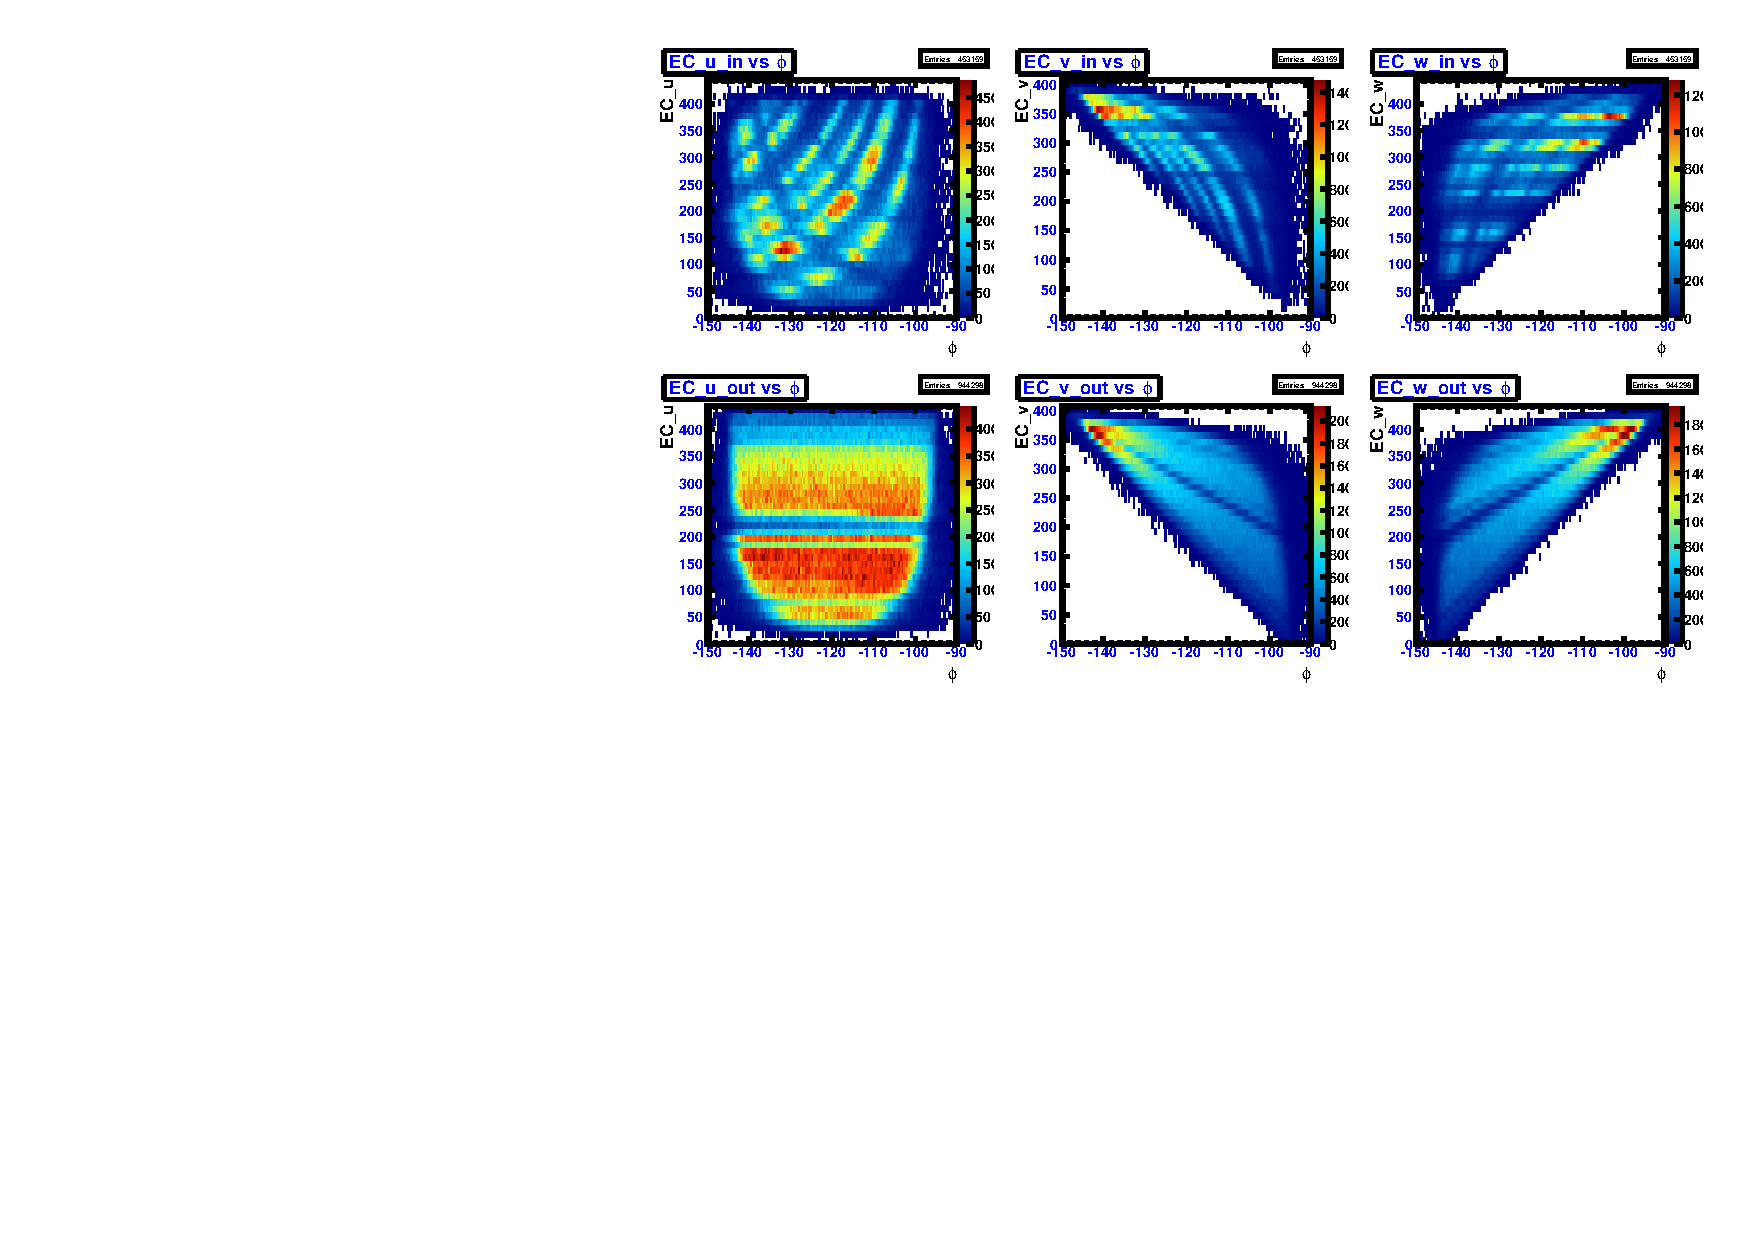
\includegraphics[width=\figwidth,height=\hfigheight]{\grpath/analysis/FIDUCIAL_CUTS/EC/pim_ecuvw_phi_NOKnockout_sec5.pdf}
\caption[Inefficient \abbr{EC} $u$, $v$, $w$ strips vs. $\phi$ for sector 5 in \abbr{CLAS} $e^{-} \ $ data]{\label{fig:neg:ec.sec5}Inefficient \abbr{EC} $u$, $v$, $w$ strips vs. $\phi$ for sector 5 in \abbr{CLAS} $e^{-} \ $ data. Top row depicts the $u$, $v$, $w$ strips for the \emph{inner} \abbr{EC}, while the bottom row depicts the $u$, $v$, $w$ strips for the \emph{outer} \abbr{EC}. The z-axis illustrates the number of hits in the plot.}
\end{center}\end{figure}
%
The projection of Fig.~\ref{fig:neg:ec.sec5} onto the y-axis can be seen in Fig.~\ref{fig:neg.ecstrip.sec5}. This view depicts the actual paddles that are dead or inefficient. It can be seen in either Figs.~\ref{fig:neg:ec.sec5} and~\ref{fig:neg.ecstrip.sec5} that there exists inefficient \abbr{EC} strips for sector 5. 
\begin{figure}[h!]\begin{center}
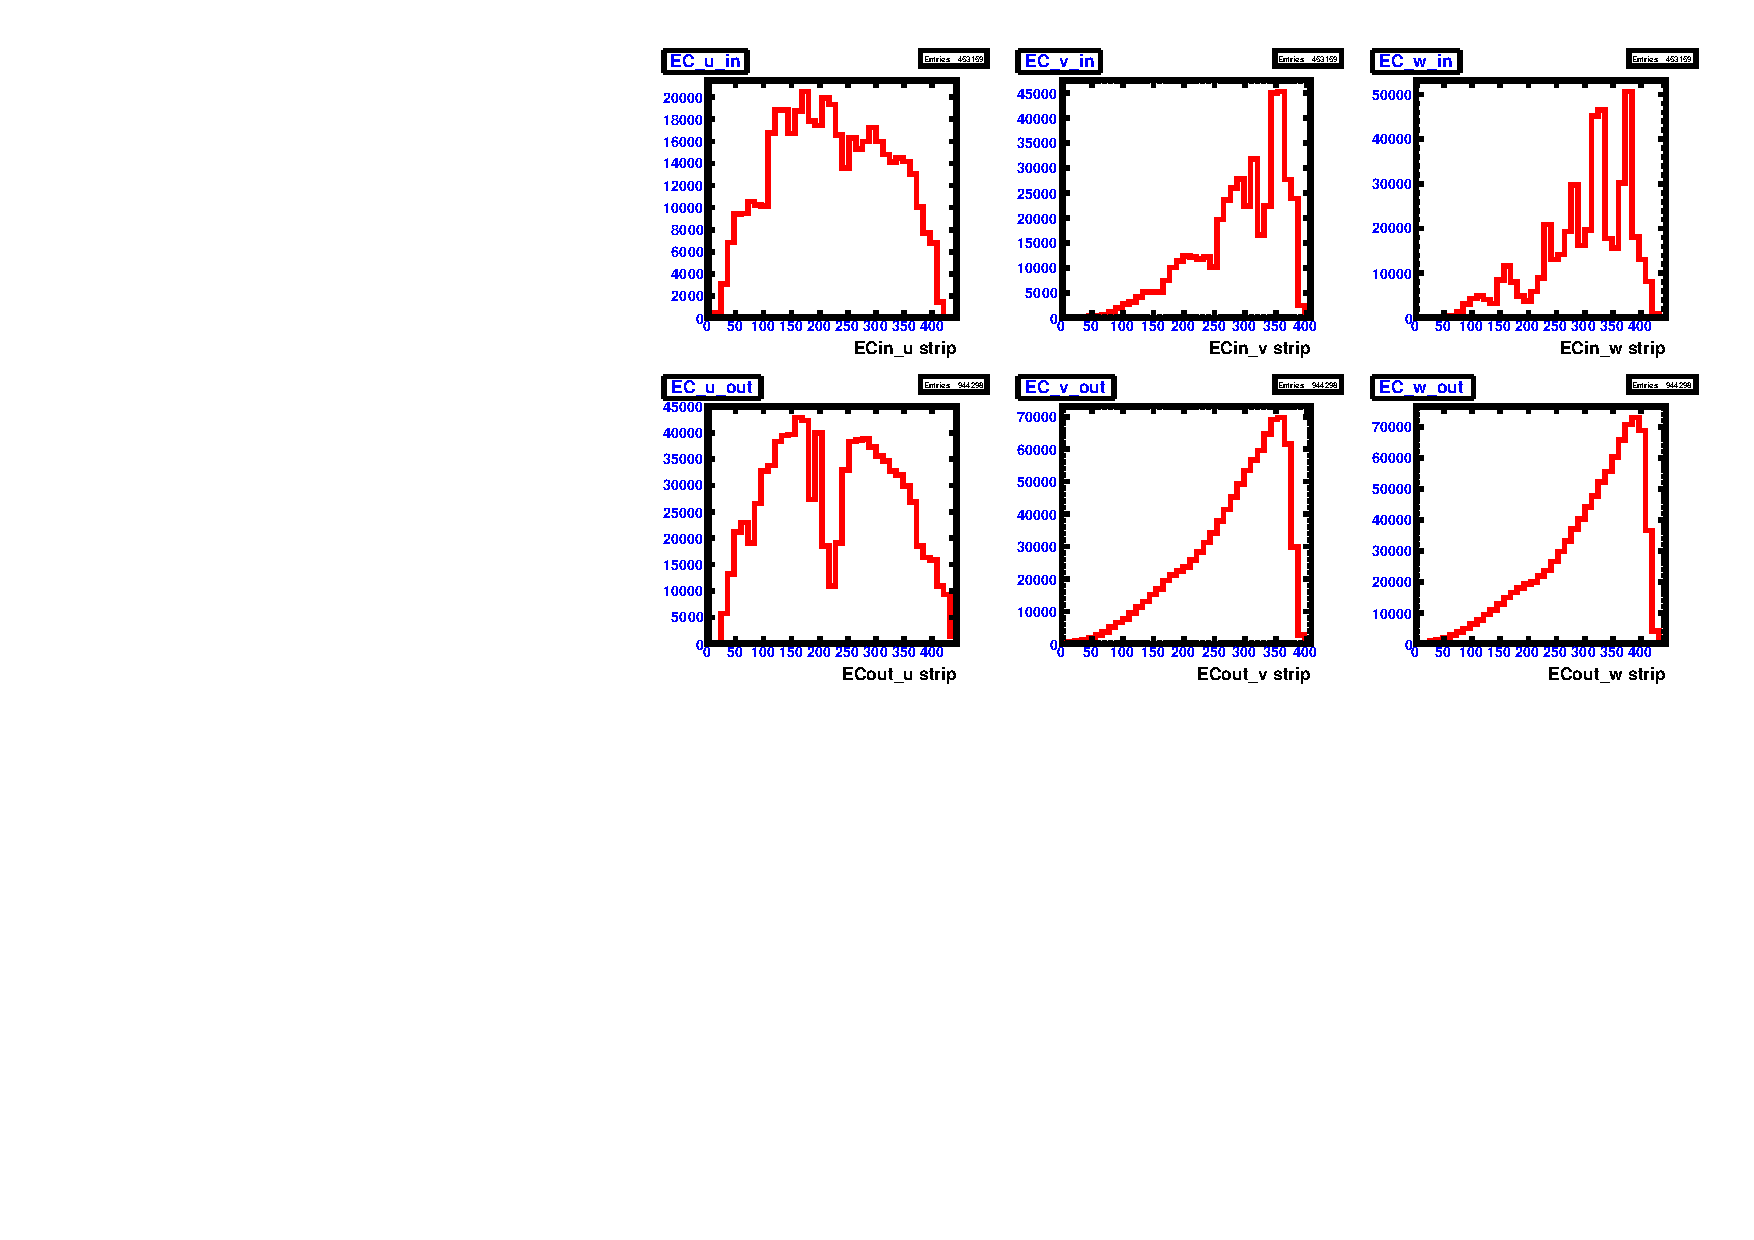
\includegraphics[width=\figwidth,height=\hfigheight]{\grpath/analysis/FIDUCIAL_CUTS/EC/pim_ecuvw_NOKnockout_sec5.pdf}
\caption[Number of hit vs. inefficient \abbr{EC} $u$, $v$, $w$ strips for sector 5 for $e^-$ data]{\label{fig:neg.ecstrip.sec5} Number of hit vs. inefficient \abbr{EC} $u$, $v$, $w$ strips for sector 5 for $e^-$ data. Top row depicts the $u$, $v$, $w$  strips for the \emph{inner} \abbr{EC}, while the bottom row depicts the $u$, $v$, $w$  strips for the \emph{outer} \abbr{EC}}
\end{center}\end{figure}
The inefficient strips were removed in data and \abbr{MC}. The effect of the inefficient strip cut, along with the standard \abbr{CLAS} \abbr{EC} geometric fiducial cuts can be seen in Fig.~\ref{fig:neg:ec.sec5_cut} and Fig.~\ref{fig:neg.ecstrip.sec5_cut}.
%
There also existed an inefficiency in other sectors. The plots to show the total inefficiency of the \abbr{EC} can be found in App.~\ref{sec:app.tof_plots}. The parameters for the \abbr{EC} strip cuts are listed in Tab.~\ref{tab:ec.eq} and the parameters for the good \abbr{EC} fiducial range can be found in Tab.~\ref{tab:ecfid.eq}.
\begin{table}[h!]
\begin{minipage}{\textwidth}
\begin{center}
\begin{singlespacing}

\caption[\abbr{EC} UVW Cut Parameters]{\label{tab:ec.eq} \abbr{EC} UVW cut parameters.}
\begin{tabular}{c|c|c}
\hline												
Sector & \abbr{EC}$_{\mathrm{\emph{inner/outer}}}$	& U  \\ \hline 	
2 & \abbr{EC}$_{\mathrm{\emph{inner}}}$ & $96\le U\le 108  \ || \  324\le U\le 336 $   \\
3 & \abbr{EC}$_{\mathrm{\emph{inner}}}$ & $324\le U\le 336  \ || \  180\le U\le 216  \ || \  324\le U\le 337 $  \\
%
2 & \abbr{EC}$_{\mathrm{\emph{outer}}}$ & $324\le U\le 336.$ \\
3 & \abbr{EC}$_{\mathrm{\emph{outer}}}$ & $131\le U\le 142  \ || \  204\le U\le 216  \ || \  324\le U\le 336 $ \\
5 & \abbr{EC}$_{\mathrm{\emph{outer}}}$ & $180\le U\le 192  \ || \  204\le U\le 240 $  \\
%
\hline
 & 	& V \\
\hline
5 & \abbr{EC}$_{\mathrm{\emph{inner}}}$  & $ 320\le V\le 342  \ || \  254\le V\le 242 $   \\
%
%
\hline
 & 	& W \\
\hline 
1 & \abbr{EC}$_{\mathrm{\emph{inner}}}$ & $312\le W\le 324$  \\
2 & \abbr{EC}$_{\mathrm{\emph{inner}}}$ & $396\le W\le 408$  \\
3 & \abbr{EC}$_{\mathrm{\emph{inner}}}$ & $ 396\le W\le 408$  \\
5 & \abbr{EC}$_{\mathrm{\emph{inner}}}$ & $ 336\le W\le 372  \ || \  288\le W\le 312  \ || \  240\le W\le 276$ \\ 
& & $  \ || \  168\le W\le 228  \ || \  132\le W\le 144$  \\
6 & \abbr{EC}$_{\mathrm{\emph{inner}}}$ & $ W\ge 396$  \\

\hline \hline%inserts single line
\end{tabular}

\end{singlespacing}
\end{center}
\end{minipage}
\end{table}
\vspace{20pt}  
\begin{table}[h!]
\begin{minipage}{\textwidth}
\begin{center}
\begin{singlespacing}

\caption[\abbr{EC} UVW Good Fiducial Parameters]{\label{tab:ecfid.eq} \abbr{EC} UVW good fiducial parameters.}
\begin{tabular}{c|c|c|c}
\hline												
\abbr{EC} Good Fiducial Range & U & V & W  \\ \hline 
& $20\le U\le 400 $  & $V\le 375.0$ & $W\le 405.0$ \\
\hline \hline%inserts single line
\end{tabular}
\end{singlespacing}
\end{center}
\end{minipage}
\end{table}
\vspace{20pt}  

\begin{figure}[h!]\begin{center}
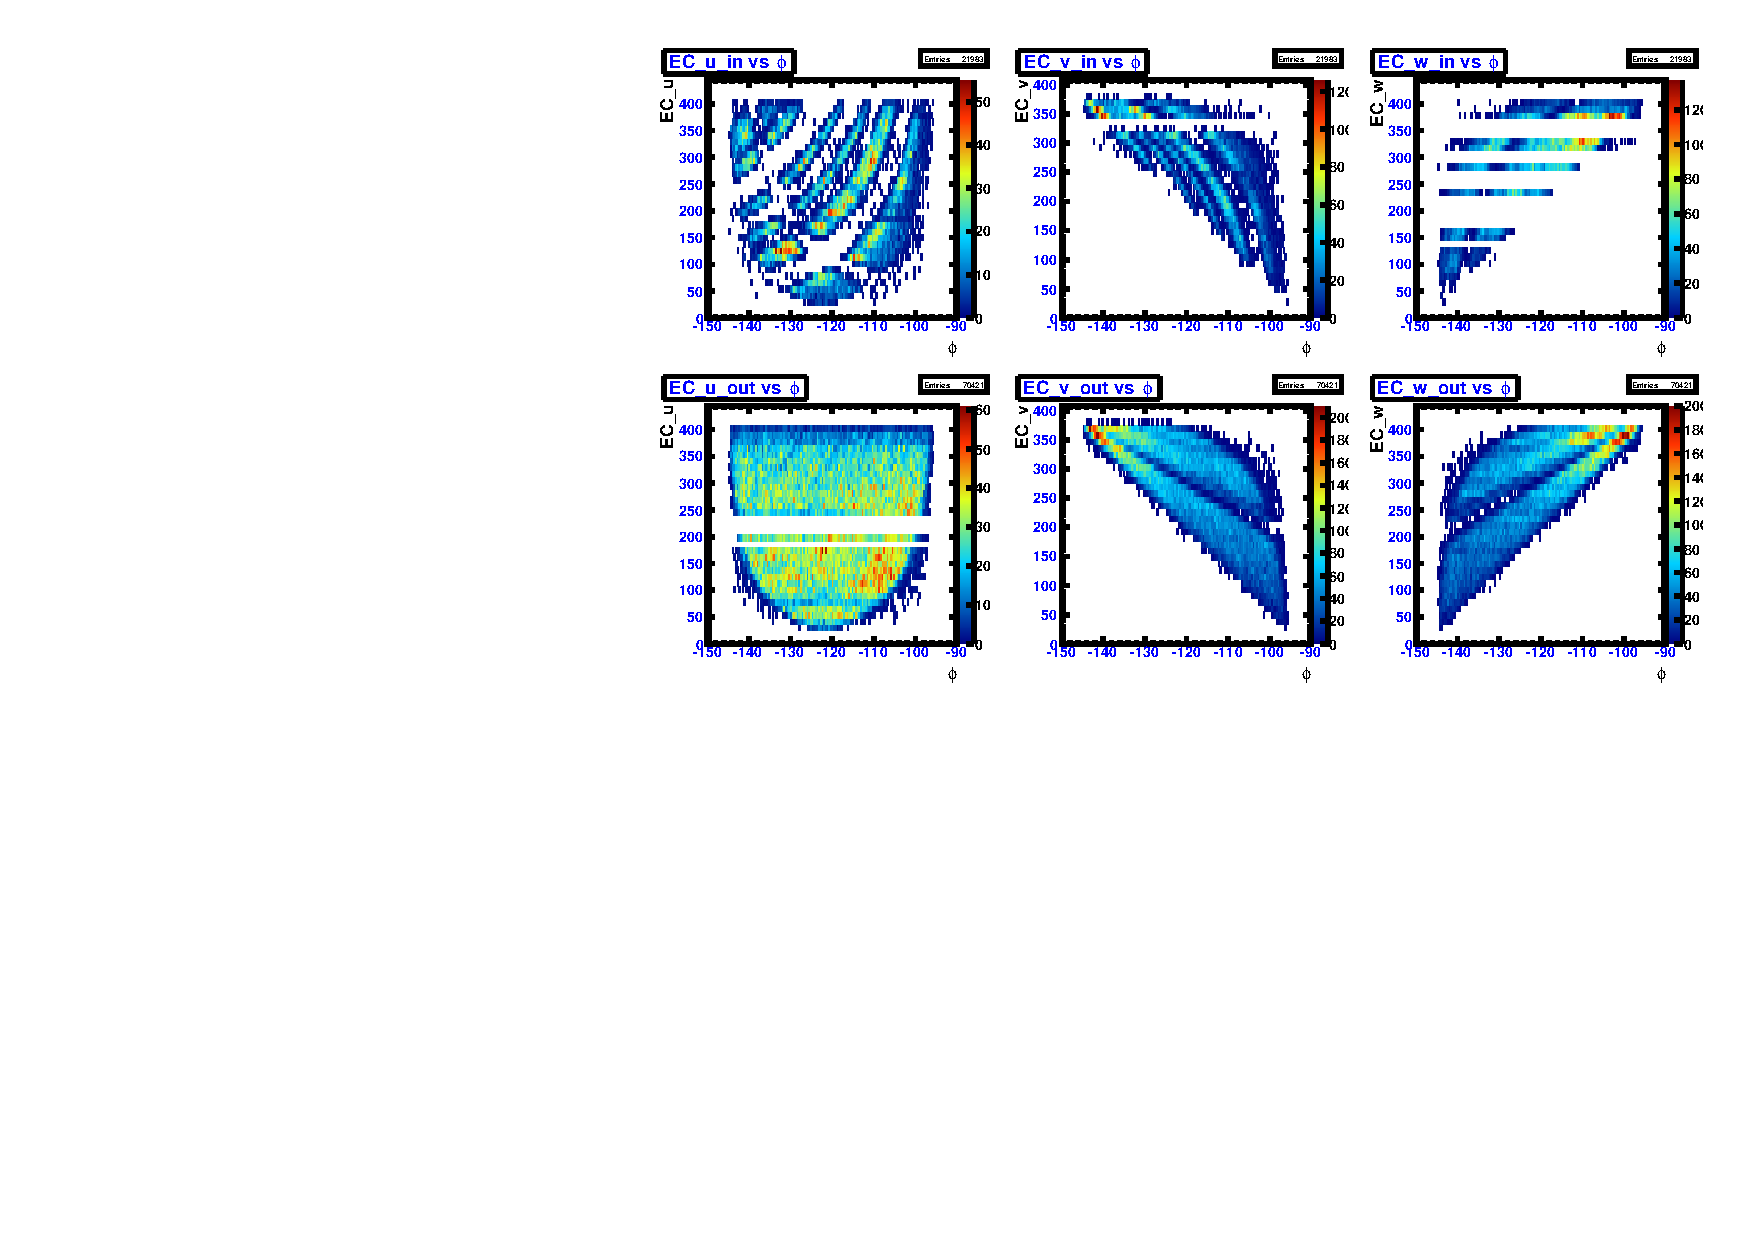
\includegraphics[width=\figwidth,height=\hfigheight]{\grpath/analysis/FIDUCIAL_CUTS/EC/pim_ecuvw_phi_afterGeoFid_sec5.pdf}
\caption[\abbr{EC} $u$, $v$, $w$ strips vs. $\phi$ for sector 5 with fiducial cuts and inefficient paddle knockouts applied to $e^-$ data]{\label{fig:neg:ec.sec5_cut} \abbr{EC} $u$, $v$, $w$ strips vs. $\phi$ for sector 5 with fiducial cuts and inefficient paddle knockouts applied to $e^-$ data. Top row depicts the $u$, $v$, $w$ strips for the \emph{inner} \abbr{EC}, while the bottom row depicts the $u$, $v$, $w$ strips for the \emph{outer} \abbr{EC}. The z-axis illustrates the number of hits in the plot.}
\end{center}\end{figure}
%
\begin{figure}[h!]\begin{center}
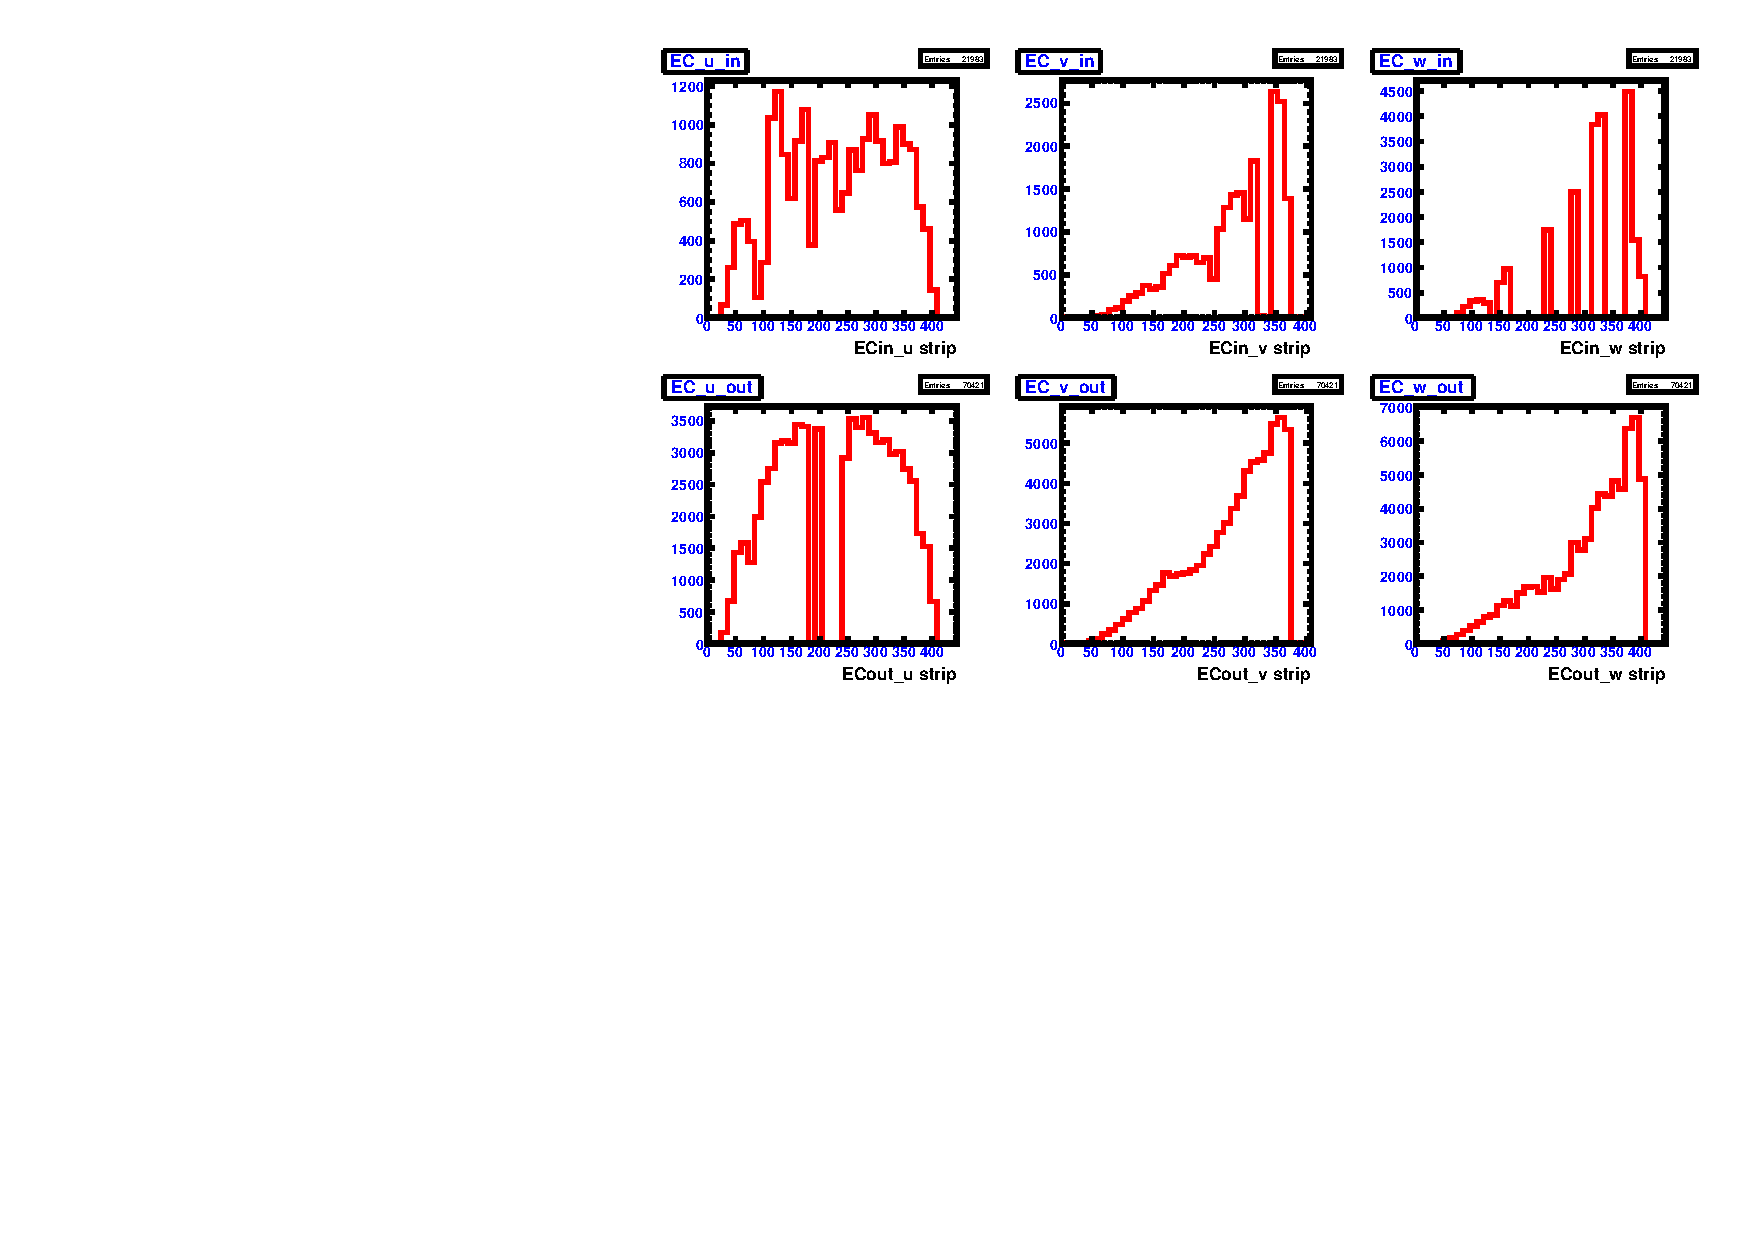
\includegraphics[width=\figwidth,height=\hfigheight]{\grpath/analysis/FIDUCIAL_CUTS/EC/pim_ecuvw_afterGeoFid_sec5.pdf}
\caption[Number of hits vs. \abbr{EC} $u$, $v$, $w$ strips for sector 5 with fiducial cuts and inefficient paddle knockouts applied to $e^-$ data]{\label{fig:neg.ecstrip.sec5_cut}Number of hits vs. \abbr{EC} $u$, $v$, $w$ strips for sector 5 with fiducial cuts and inefficient paddle knockouts applied to $e^-$ data. Top row depicts the $u$, $v$, $w$ strips for the \emph{inner} \abbr{EC}, while the bottom row depicts the $u$, $v$, $w$ strips for the \emph{outer} \abbr{EC}}
\end{center}\end{figure}

\FloatBarrier